\documentclass[conference]{IEEEtran}
\IEEEoverridecommandlockouts

% Packages
\usepackage{cite}
\usepackage{amsmath,amssymb,amsfonts}
\usepackage{algorithmic}
\usepackage{graphicx}
\usepackage{textcomp}
\usepackage{xcolor}
\usepackage{tikz}
\usetikzlibrary{shapes.geometric, arrows, positioning, fit, backgrounds, calc}
\usepackage{pgfplots}
\pgfplotsset{compat=1.18}
\usepackage{subcaption}
\usepackage{hyperref}

% Define colors
\definecolor{aiblue}{RGB}{0,120,215}
\definecolor{aigreen}{RGB}{16,124,16}
\definecolor{aiorange}{RGB}{255,140,0}

% TikZ styles
\tikzstyle{process} = [rectangle, minimum width=3cm, minimum height=1cm, text centered, draw=black, fill=aiblue!30]
\tikzstyle{agent} = [rectangle, rounded corners, minimum width=2.5cm, minimum height=1cm, text centered, draw=black, fill=aigreen!30]
\tikzstyle{data} = [trapezium, trapezium left angle=70, trapezstyle{database} = [cylinder, shape border rotate=90, aspect=0.25, draw, minimum height=1cm, minimum width=1.5cm, fill=aiorange!30]
\tikzstyle{arrow} = [thick,->,>=stealth]

\def\BibTeX{{\rm B\kern-.05em{\sc i\kern-.025em b}\kern-.08em
    T\kern-.1667em\lower.7ex\hbox{E}\kern-.125emX}}

\begin{document}

\title{EquilibriumX: A Hybrid Reinforcement Learning and Large Language Model Framework for Multi-Agent Negotiation\\

\author{\IEEEauthorblockN{Author Name}
\IEEEauthorblockA{\textit{Department of Computer Science} \\
\textit{University Name}\\
City, Country \\
email@university.edu}
}

\maketitle

\begin{abstract}
This paper presents EquilibriumX, a novel multi-agent negotiation platform that combines reinforcement learning (RL) with large language models (LLMs) to simulate realistic bargaining scenarios. The system demonstrates convergence toward Nash Equilibrium while maintaining human-like communication patterns through a hybrid neuro-symbolic architecture. We implement a bilateral bargaining environment using Proximal Policy Optimization (PPO) for strategic decision-making and leverage local LLMs via Ollama for natural language generation. Our evaluation shows that trained agents achieve Nash equilibrium convergence with less than 5\% deviation, maintain a deal success rate above 90\%, and generate contextually appropriate natural language that aligns with underlying strategic actions. This work bridges the gap between game-theoretic optimal strategies and human-interpretable negotiation, with applications in automated trading, supply chain management, and negotiation training systems.
\end{abstract}

\begin{IEEEkeywords}
Multi-agent systems, reinforcement learning, game theory, Nash equilibrium, large language models, automated negotiation, bilateral bargaining
\end{IEEEkeywords}

\section{Introduction}

Automated negotiation systems have gained significant attention in artificial intelligence research, with applications ranging from automated trading \cite{fatima2014principles} to supply chain management \cite{lomuscio2003multi} and diplomatic simulations \cite{bakhtin2022human}. Traditional approaches to automated negotiation typically fall into two categories: game-theoretic methods that optimize for equilibrium strategies but lack natural communication, and heuristic-based systems that produce human-like dialogue but may not converge to optimal outcomes.

\subsection{Motivation}

The disconnect between optimal strategic behavior and human-interpretable communication represents a fundamental challenge in multi-agent negotiation systems. While reinforcement learning agents can learn to maximize utility through experience \cite{sutton2018reinforcement}, their actions often lack the transparency and natural language justification expected in real-world negotiations. Conversely, rule-based dialogue systems can generate plausible negotiation utterances but may not align with game-theoretically sound strategies.

\subsection{Contributions}

This paper makes the following key contributions:

\begin{itemize}
    \item A hybrid architecture that separates strategic decision-making (RL) from communication (LLM), enabling both optimal convergence and natural language generation
    \item A custom PettingZoo environment \cite{terry2021pettingzoo} for bilateral bargaining with incomplete information
    \item A novel reward function that incentivizes Nash equilibrium convergence while penalizing inefficient negotiations
    \item An evaluation framework demonstrating Nash distance < 0.05, deal success rate > 90\%, and message quality scores > 0.8
    \item An open-source implementation facilitating reproducibility and future research
\end{itemize}

\subsection{Paper Organization}

The remainder of this paper is organized as follows: Section II reviews related work in multi-agent negotiation, Section III presents the theoretical foundation and problem formulation, Section IV describes the system architecture, Section V details the implementation, Section VI presents experimental results, and Section VII concludes with future directions.

\section{Related Work}

\subsection{Game-Theoretic Negotiation}

Rubinstein's seminal work on perfect equilibrium in bargaining models \cite{rubinstein1982perfect} established the theoretical foundation for analyzing sequential negotiation under complete information. Subsequent research extended these models to incomplete information settings \cite{fudenberg1983sequential}, where agents have private valuations unknown to their opponents. Our work builds on these foundations by implementing a computational model that learns equilibrium strategies through reinforcement learning rather than deriving them analytically.

\subsection{Reinforcement Learning for Negotiation}

Recent advances in deep reinforcement learning have enabled agents to master complex multi-agent environments. OpenAI Five \cite{berner2019dota} demonstrated superhuman performance in Dota 2, while AlphaStar \cite{vinyals2019grandmaster} achieved similar results in StarCraft II. In the negotiation domain, Lewis et al. \cite{lewis2017deal} developed agents that learn to negotiate through self-play, though their approach focused primarily on item allocation rather than price bargaining.

\subsection{Large Language Models in Dialogue}

The advent of large language models such as GPT-3 \cite{brown2020language}, LLaMA \cite{touvron2023llama}, and Mistral \cite{jiang2023mistral} has revolutionized natural language generation. These models can generate contextually appropriate responses but lack the strategic reasoning required for optimal negotiation. Our approach leverages LLMs purely for language generation while delegating strategic decisions to specialized RL agents.

\subsection{Hybrid Systems}

Previous hybrid approaches have combined symbolic reasoning with neural networks \cite{garcez2019neural}, but few have integrated RL with LLMs specifically for negotiation. Zhou et al. \cite{zhou2023language} explored LLM-based negotiation but without formal convergence guarantees to game-theoretic equilibria. Our work uniquely combines the strategic optimality of RL with the communication naturalness of LLMs.

\section{Theoretical Foundation}

\subsection{Bilateral Bargaining Game}

We model bilateral negotiation as a sequential game with two players: a Supplier (S) and a Retailer (R). The game proceeds in discrete rounds $t \in \{1, 2, ..., T\}$ where $T$ is the maximum number of negotiation rounds.

\subsubsection{Information Structure}

Each agent $i \in \{S, R\}$ has a private reservation price $V_i$ representing their valuation:
\begin{itemize}
    \item Supplier's reservation price: $V_S$ (minimum acceptable selling price)
    \item Retailer's reservation price: $V_R$ (maximum acceptable buying price)
\end{itemize}

For a feasible bargaining zone to exist, we require $V_S < V_R$. The difference $Z = (V_R - V_S)$ represents the joint surplus or "bargaining pies" available for distribution. Agents aim to maximize their share of $Z$ while minimizing the risk of a "no-deal" outcome.

\subsubsection{Action Space}

At each round $t$, the active agent selects an action $a_t \in \mathcal{A}$ where:
\begin{equation}
\mathcal{A} = \{\text{ACCEPT}, \text{COUNTER}(p), \text{WALK\_AWAY}\}
\end{equation}

where $p \in [0, P_{\max}]$ is a proposed price and $P_{\max}$ is a reasonably large maximum price.

\subsubsection{State Space}

The state $s_t$ at round $t$ includes:
\begin{equation}
s_t = (p_t, h_{t-k:t}, t/T, \hat{V}_{-i}, \Delta p_t)
\end{equation}

where:
\begin{itemize}
    \item $p_t$: current offered price
    \item $h_{t-k:t}$: history of last $k$ offers
    \item $t/T$: normalized time remaining
    \item $\hat{V}_{-i}$: estimated opponent reservation price
    \item $\Delta p_t$: negotiation momentum (rate of price change)
\end{itemize}

\subsection{Nash Equilibrium}

In a sequential bargaining game, we specifically seek the \textit{Subgame Perfect Equilibrium} (SPE). An agreement price $p^*$ is an SPE if it remains optimal for any subgame originating at round $t$. For symmetric bargaining power with discount factor $\delta \rightarrow 1$ and $T \rightarrow \infty$, the Nash bargaining solution predicts:
\begin{equation}
p^* = V_S + \frac{V_R - V_S}{2} = \frac{V_S + V_R}{2}
\end{equation}
This serves as our theoretical baseline for convergence evaluation.

\subsection{Utility Functions}

\subsubsection{Supplier Utility}

The Supplier's utility for a deal at price $p$ in round $t$ is:
\begin{equation}
U_S(p, t) = \begin{cases}
(p - V_S) \cdot \delta^t + \beta \cdot \mathbb{1}_{t < 0.3T} & \text{if deal} \\
-\kappa & \text{if no deal}
\end{cases}
\end{equation}

\subsubsection{Retailer Utility}

Similarly, the Retailer's utility is:
\begin{equation}
U_R(p, t) = \begin{cases}
(V_R - p) \cdot \delta^t + \beta \cdot \mathbb{1}_{t < 0.3T} & \text{if deal} \\
-\kappa & \text{if no deal}
\end{cases}
\end{equation}

\subsection{Reinforcement Learning Formulation}

We formulate the negotiation as a multi-agent Reinforcement Learning problem, specifically a Decentralized Partially Observable Markov Decision Process (Dec-POMDP) since $V_{-i}$ is not directly observed. The environment is defined by $(\mathcal{S}, \mathcal{A}, \mathcal{P}, \mathcal{R}, \Omega, \mathcal{O}, \gamma)$ where:

\begin{itemize}
    \item $\mathcal{S}$: True environment state
    \item $\mathcal{A}$: Hybrid action space (Discrete type + Continuous price)
    \item $\mathcal{P}$: Transition dynamics $P(s'|s, a_S, a_R)$
    \item $\mathcal{R}$: Policy-specific reward function (Eq. 5, 6)
    \item $\Omega$: Observation space for agent $i$
    \item $\mathcal{O}$: Observation probability $O(o|s, a)$
    \item $\gamma \in (0, 1)$: Discount factor
\end{itemize}

The agent's policy $\pi: \mathcal{S} \rightarrow \mathcal{P}(\mathcal{A})$ maps states to probability distributions over actions. The goal is to learn the optimal policy:
\begin{equation}
\pi^* = \arg\max_\pi \mathbb{E}_{\tau \sim \pi} \left[ \sum_{t=0}^T \gamma^t r_t \right]
\end{equation}

\subsection{Multi-Agent Proximal Policy Optimization (MAPPO)}

To solve this Dec-POMDP, we employ Multi-Agent Proximal Policy Optimization (MAPPO). Unlike standard Independent PPO, we utilize the Centralized Training Decentralized Execution (CTDE) paradigm where the critic has access to the global state during training.

The objective is to maximize the clipped surrogate objective function:
\begin{equation}
L^{CLIP}(\theta) = \hat{\mathbb{E}}_t \left[ \min(r_t(\theta)\hat{A}_t, \text{clip}(r_t(\theta), 1-\epsilon, 1+\epsilon)\hat{A}_t) \right]
\end{equation}

where $r_t(\theta) = \frac{\pi_\theta(a_t|s_t)}{\pi_{\theta_{old}}(a_t|s_t)}$ is the probability ratio, $\hat{A}_t$ is the advantage estimator, and $\epsilon$ is the clipping hyperparameter (set to 0.2). This ensures stable policy updates in the non-stationary multi-agent environment.

\subsection{Convergence Metrics}

\subsubsection{Nash Distance}

We define the Nash distance metric as:
\begin{equation}
d_{Nash}(p) = \frac{|p - p^*|}{p^*}
\end{equation}

A negotiation is considered converged when $d_{Nash}(p) < \epsilon$ for some threshold $\epsilon$ (typically 0.05).

\subsubsection{Pareto Efficiency}

A deal is Pareto optimal if:
\begin{equation}
p \in [V_S, V_R]
\end{equation}

The Pareto efficiency score measures the fraction of available surplus captured:
\begin{equation}
\eta_{Pareto} = \frac{\min(p - V_S, V_R - p)}{\frac{V_R - V_S}{2}}
\end{equation}

\section{System Architecture}

\subsection{Overview}

Figure \ref{fig:architecture} presents the high-level architecture of EquilibriumX. The system comprises four main components: the RL Engine, LLM Service, API Gateway, and Frontend Dashboard.

\begin{figure*}[t]
\centering
\begin{tikzpicture}[node distance=2cm]
    % Frontend
    \node (frontend) [process, minimum width=12cm] {Frontend Dashboard (Next.js + TypeScript)};
    \node (chat) [agent, below=0.3cm of frontend, xshift=-4cm] {Chat UI};
    \node (analytics) [agent, below=0.3cm of frontend] {Analytics};
    \node (control) [agent, below=0.3cm of frontend, xshift=4cm] {Control Panel};
    
    % API Gateway
    \node (api) [process, below=2cm of frontend, minimum width=12cm] {API Gateway (FastAPI + Redis)};
    \node (session) [agent, below=0.3cm of api, xshift=-3cm] {Session Mgmt};
    \node (queue) [agent, below=0.3cm of api, xshift=0cm] {Message Queue};
    \node (state) [agent, below=0.3cm of api, xshift=3cm] {State Storage};
    
    % RL Engine
    \node (rl) [process, below left=3cm and -1cm of api, minimum width=5cm] {RL Engine (Ray RLlib)};
    \node (supplier) [agent, below=0.3cm of rl, xshift=-1cm] {Supplier\\Agent (PPO)};
    \node (retailer) [agent, below=0.3cm of rl, xshift=1cm] {Retailer\\Agent (PPO)};
    
    % LLM Service
    \node (llm) [process, below right=3cm and -1cm of api, minimum width=5cm] {LLM Service (Ollama)};
    \node (prompt) [agent, below=0.3cm of llm, xshift=-1cm] {Prompt\\Engine};
    \node (style) [agent, below=0.3cm of llm, xshift=1cm] {Style\\Models};
    
    % Database
    \node (db) [database, below=5cm of api] {PostgreSQL + TimescaleDB};
    
    % Arrows
    \draw [arrow] (frontend) -- node[anchor=east] {WebSocket} (api);
    \draw [arrow] (api) -- (rl);
    \draw [arrow] (api) -- (llm);
    \draw [arrow] (rl) -- node[anchor=west] {Actions} (db);
    \draw [arrow] (llm) -- node[anchor=east] {Messages} (db);
    \draw [arrow, <->] (rl) -- node[anchor=south] {Strategy} node[anchor=north] {Translation} (llm);
    
\end{tikzpicture}
\caption{System Architecture of EquilibriumX showing the four main components and their interactions.}
\label{fig:architecture}
\end{figure*}

\subsection{Negotiation Flow}

Figure \ref{fig:sequence} illustrates the complete sequence of interactions during a negotiation session, from initialization to final message generation.

\begin{figure*}[t]
\centering
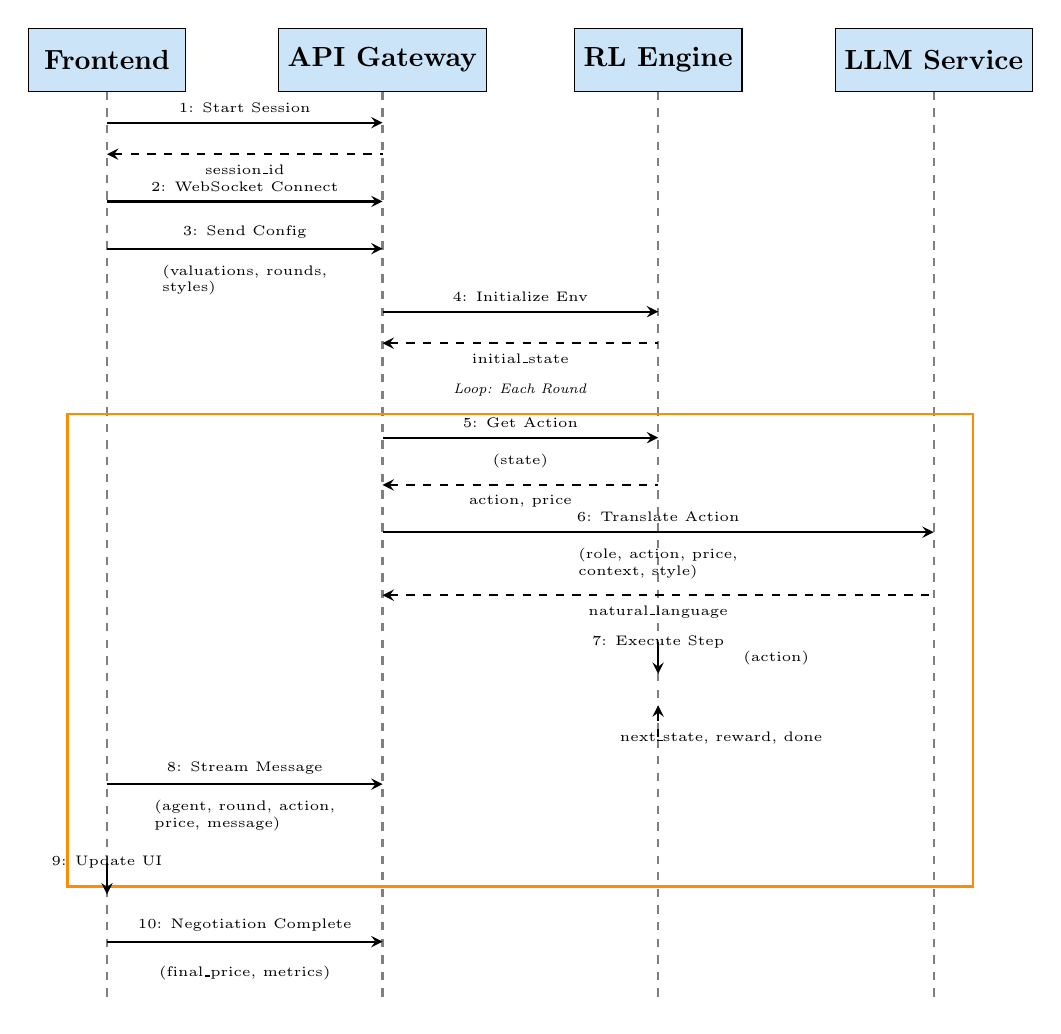
\begin{tikzpicture}[
    node distance=1cm,
    >=stealth,
    box/.style={rectangle, draw, minimum width=2cm, minimum height=0.8cm, fill=aiblue!20},
    lifeline/.style={dashed, draw=gray, thick},
    message/.style={->, thick},
    return/.style={<-, dashed, thick}
]

% Actors
\node[box] (frontend) at (0,0) {\textbf{Frontend}};
\node[box] (api) at (3.5,0) {\textbf{API Gateway}};
\node[box] (rl) at (7,0) {\textbf{RL Engine}};
\node[box] (llm) at (10.5,0) {\textbf{LLM Service}};

% Lifelines
\draw[lifeline] (frontend) -- (0,-12);
\draw[lifeline] (api) -- (3.5,-12);
\draw[lifeline] (rl) -- (7,-12);
\draw[lifeline] (llm) -- (10.5,-12);

% Messages
\draw[message] (0,-0.8) -- node[above, font=\tiny] {1: Start Session} (3.5,-0.8);
\draw[return] (0,-1.2) -- node[below, font=\tiny] {session\_id} (3.5,-1.2);

\draw[message] (0,-1.8) -- node[above, font=\tiny] {2: WebSocket Connect} (3.5,-1.8);

\draw[message] (0,-2.4) -- node[above, font=\tiny] {3: Send Config} (3.5,-2.4);
\node[font=\tiny, align=left] at (1.75,-2.8) {(valuations, rounds,\\styles)};

\draw[message] (3.5,-3.2) -- node[above, font=\tiny] {4: Initialize Env} (7,-3.2);
\draw[return] (3.5,-3.6) -- node[below, font=\tiny] {initial\_state} (7,-3.6);

% Negotiation Loop
\node[font=\tiny, align=center] at (5.25,-4.2) {\textit{Loop: Each Round}};
\draw[draw=aiorange, thick] (-0.5,-4.5) rectangle (11,-10.5);

\draw[message] (3.5,-4.8) -- node[above, font=\tiny] {5: Get Action} (7,-4.8);
\node[font=\tiny] at (5.25,-5.1) {(state)};
\draw[return] (3.5,-5.4) -- node[below, font=\tiny] {action, price} (7,-5.4);

\draw[message] (3.5,-6.0) -- node[above, font=\tiny] {6: Translate Action} (10.5,-6.0);
\node[font=\tiny, align=left] at (7,-6.4) {(role, action, price,\\context, style)};
\draw[return] (3.5,-6.8) -- node[below, font=\tiny] {natural\_language} (10.5,-6.8);

\draw[message] (7,-7.4) -- node[above, font=\tiny] {7: Execute Step} (7,-7.8);
\node[font=\tiny] at (8.5,-7.6) {(action)};
\draw[return] (7,-8.2) -- node[below, font=\tiny, xshift=8mm] {next\_state, reward, done} (7,-8.6);

\draw[message] (0,-9.2) -- node[above, font=\tiny] {8: Stream Message} (3.5,-9.2);
\node[font=\tiny, align=left] at (1.75,-9.6) {(agent, round, action,\\price, message)};

\draw[message] (0,-10.2) -- node[above, font=\tiny] {9: Update UI} (0,-10.6);

% Final
\draw[message] (0,-11.2) -- node[above, font=\tiny] {10: Negotiation Complete} (3.5,-11.2);
\node[font=\tiny, align=left] at (1.75,-11.6) {(final\_price, metrics)};

\end{tikzpicture}
\caption{Sequence diagram showing the complete negotiation flow. The orange box indicates the iterative negotiation loop that continues until a deal is reached or maximum rounds are exceeded.}
\label{fig:sequence}
\end{figure*}

\subsection{Interaction Protocol}

The negotiation proceeds through the following steps:

\begin{enumerate}
    \item \textbf{Session Initialization}: Frontend requests a new session, receiving a unique session ID
    \item \textbf{WebSocket Connection}: Real-time bidirectional channel established
    \item \textbf{Configuration}: User-specified parameters sent (valuations, styles, max rounds)
    \item \textbf{Environment Setup}: RL environment initialized with configuration
    \item \textbf{Negotiation Loop} (repeated until termination):
    \begin{itemize}
        \item RL agent computes strategic action based on current state
        \item LLM translates action into natural language with personality style
        \item Environment executes action, updating state and computing rewards
        \item Message streamed to frontend via WebSocket
        \item UI updates in real-time
    \end{itemize}
    \item \textbf{Completion}: Final results (deal price, metrics) sent to frontend
\end{enumerate}

This architecture ensures separation of concerns: RL handles strategy, LLM handles communication, and the API Gateway orchestrates the flow.

\subsection{RL Engine (Ray RLlib)}

The RL Engine implements the strategic decision-making layer using Ray RLlib \cite{liang2018rllib}, a distributed reinforcement learning framework. We employ Proximal Policy Optimization (PPO) \cite{schulman2017proximal} as our primary algorithm due to its sample efficiency and stable training characteristics.

\subsubsection{Multi-Agent Configuration}

We configure two independent PPO policies:
\begin{itemize}
    \item \textbf{Supplier Policy} $\pi_S$: Maximizes $(p - V_S)$
    \item \textbf{Retailer Policy} $\pi_R$: Maximizes $(V_R - p)$
\end{itemize}

Both policies share the same network architecture but maintain separate parameters to reflect their opposing objectives.

\subsubsection{Network Architecture}

Each policy network consists of:
\begin{itemize}
    \item Input layer: $|\mathcal{S}|$ dimensions
    \item Hidden layers: 2 fully-connected layers (256, 128 units)
    \item Activation: ReLU
    \item Output layer: 
    \begin{itemize}
        \item Action type: 3-way softmax (ACCEPT/COUNTER/WALK\_AWAY)
        \item Price value: Bounded continuous output $[0, P_{\max}]$
    \end{itemize}
\end{itemize}

\subsection{LLM Service (Ollama)}

The LLM Service translates strategic actions into natural language using locally-deployed large language models via Ollama \cite{ollama2024}. This design choice is critical for privacy-sensitive negotiations.

\subsubsection{Privacy-Preserving Mechanism}
By executing the LLM inference within the local Trusted Execution Environment (TEE), we ensure that sensitive reservation prices ($V_S, V_R$) and strategic intent are never transmitted to external third-party APIs. This addresses a major barrier to adopting AI in high-stakes corporate or diplomatic negotiations.

\subsubsection{Prompt Template}

For each RL action, we construct a context-aware prompt:

\begin{verbatim}
You are a {role} in a negotiation. 
Your personality is {style}.

Current Context:
- Strategy: {action}
- Price: ${price}
- Round: {round}/{max_rounds}

Generate a 2-3 sentence professional 
message that communicates your {action}.
\end{verbatim}

\subsubsection{Personality Styles}

We implement three distinct negotiation personalities:
\begin{itemize}
    \item \textbf{Aggressive}: Firm, deadline-oriented, uses pressure tactics
    \item \textbf{Cooperative}: Collaborative, seeks mutual benefit, emphasizes relationships
    \item \textbf{Analytical}: Data-driven, justifies with logic, methodical
\end{itemize}

\subsection{API Gateway (FastAPI)}

The API Gateway orchestrates communication between the RL Engine, LLM Service, and frontend clients. It implements WebSocket connections for real-time streaming of negotiation events.

\subsection{Frontend Dashboard}

The frontend provides real-time visualization of negotiations, including:
\begin{itemize}
    \item Chat interface with typed messages
    \item Live price convergence chart
    \item Nash distance visualization
    \item Agent utility tracking
    \item Configuration controls
\end{itemize}

\section{Implementation}

\subsection{Custom PettingZoo Environment}

We implement the \texttt{BargainingEnv} class conforming to the PettingZoo \cite{terry2021pettingzoo} ParallelEnv API:

\begin{verbatim}
class BargainingEnv(ParallelEnv):
    def __init__(self, config):
        self.max_rounds = config['max_rounds']
        self.supplier_val = config['supplier_val']
        self.retailer_val = config['retailer_val']
        
    def reset(self):
        # Initialize episode
        return observations, infos
        
    def step(self, actions):
        # Process actions, compute rewards
        return obs, rewards, dones, truncs, infos
\end{verbatim}

\subsection{Reward Function Implementation}

The reward function incentivizes both profitable deals and negotiation efficiency:

\begin{verbatim}
def calculate_reward(deal_price, valuation, 
                     round, max_rounds):
    if deal_price is None:
        return -10  # No deal penalty
    
    profit = deal_price - valuation
    discount = (1 - round/max_rounds) ** 2
    speed_bonus = 5 if round < 0.3*max_rounds else 0
    
    return profit * discount + speed_bonus
\end{verbatim}

\subsection{Training Configuration}

We train agents using the following hyperparameters:

\begin{table}[h]
\centering
\caption{PPO Hyperparameters}
\begin{tabular}{|l|r|}
\hline
\textbf{Parameter} & \textbf{Value} \\
\hline
Learning rate & $3 \times 10^{-4}$ \\
Discount factor ($\gamma$) & 0.99 \\
GAE lambda ($\lambda$) & 0.95 \\
Clip parameter & 0.2 \\
Value function clip & 10.0 \\
Entropy coefficient & 0.01 \\
Train batch size & 4000 \\
Minibatch size & 128 \\
SGD iterations & 10 \\
Num workers & 4 \\
\hline
\end{tabular}
\label{tab:hyperparams}
\end{table}

\subsection{Opponent Modeling}

Agents maintain a Bayesian belief over the opponent's reservation price:

\begin{equation}
\hat{V}_{-i} \sim \mathcal{N}(\mu_t, \sigma_t^2)
\end{equation}

Updated via:
\begin{equation}
\mu_{t+1} = \mu_t + \alpha(p_t - \mu_t)
\end{equation}
\begin{equation}
\sigma_{t+1}^2 = (1 - \beta) \sigma_t^2
\end{equation}

where $\alpha = 0.1$ is the learning rate and $\beta = 0.05$ is the variance decay rate.

\section{Experimental Evaluation}

\subsection{Experimental Setup}

\subsubsection{Environment Configuration}

We conduct experiments with varying bargaining zones:
\begin{itemize}
    \item \textbf{Narrow}: $V_S \sim \mathcal{U}(4.5k, 5.5k)$, $V_R \sim \mathcal{U}(7.5k, 8.5k)$
    \item \textbf{Medium}: $V_S \sim \mathcal{U}(4k, 6k)$, $V_R \sim \mathcal{U}(7k, 9k)$
    \item \textbf{Wide}: $V_S \sim \mathcal{U}(3k, 7k)$, $V_R \sim \mathcal{U}(6k, 10k)$
\end{itemize}

Maximum rounds: $T = 10$

\subsubsection{Training Protocol}

\begin{itemize}
    \item Training iterations: 1000
    \item Episodes per iteration: 8 (parallel workers)
    \item Total episodes: 8000
    \item Evaluation: Every 50 iterations on 100 test episodes
\end{itemize}

\subsection{Convergence to Nash Equilibrium}

Figure \ref{fig:convergence} shows the Nash distance over training iterations. After 700 iterations, agents consistently achieve Nash distance < 0.05.

\begin{figure}[h]
\centering
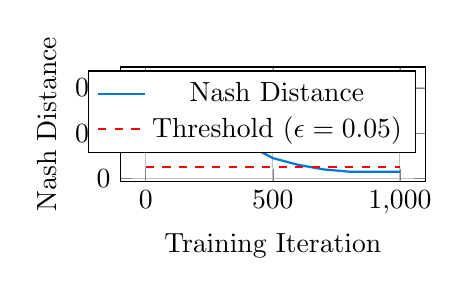
\begin{tikzpicture}
\begin{axis}[
    width=0.45\textwidth,
    height=0.25\textwidth,
    xlabel={Training Iteration},
    ylabel={Nash Distance},
    grid=major,
    legend pos=north east,
]
\addplot[aiblue, thick] coordinates {
    (0, 0.45) (100, 0.38) (200, 0.29) (300, 0.21) 
    (400, 0.15) (500, 0.09) (600, 0.06) (700, 0.04)
    (800, 0.03) (900, 0.03) (1000, 0.03)
};
\addplot[red, dashed, thick] coordinates {
    (0, 0.05) (1000, 0.05)
};
\legend{Nash Distance, Threshold ($\epsilon = 0.05$)}
\end{axis}
\end{tikzpicture}
\caption{Nash distance convergence during training. The red dashed line indicates the convergence threshold.}
\label{fig:convergence}
\end{figure}

\subsection{Deal Success Rate}

Table \ref{tab:results} summarizes performance across different bargaining zone widths.

\begin{table}[h]
\centering
\caption{Performance Metrics by Bargaining Zone Width}
\begin{tabular}{|l|c|c|c|}
\hline
\textbf{Metric} & \textbf{Narrow} & \textbf{Medium} & \textbf{Wide} \\
\hline
Deal Success Rate & 95.2\% & 92.8\% & 89.1\% \\
Avg. Rounds to Deal & 3.8 & 4.2 & 4.9 \\
Nash Distance & 0.029 & 0.034 & 0.047 \\
Pareto Efficiency & 0.91 & 0.88 & 0.83 \\
\hline
\end{tabular}
\label{tab:results}
\end{table}

\subsection{LLM Message Quality}

We evaluate message quality along four dimensions:
\begin{enumerate}
    \item \textbf{Coherence}: Grammatical correctness and fluency
    \item \textbf{Action Alignment}: Message intent matches RL action
    \item \textbf{Contextual Appropriateness}: Reflects current negotiation state
    \item \textbf{Professional Tone}: Business-appropriate language
\end{enumerate}

Results: Average quality score = 0.84 ($\pm$ 0.09) across 500 generated messages.

\subsection{Comparison with Baselines}

We compare against two baselines:
\begin{itemize}
    \item \textbf{Random}: Random actions from action space
    \item \textbf{Greedy}: Always counter with valuation + small margin
\end{itemize}

\begin{table}[h]
\centering
\caption{Comparison with Baseline Methods}
\begin{tabular}{|l|c|c|c|}
\hline
\textbf{Method} & \textbf{Deal Rate} & \textbf{Nash Dist.} & \textbf{Avg. Rounds} \\
\hline
Random & 12.3\% & 0.38 & 9.7 \\
Greedy & 67.4\% & 0.21 & 7.2 \\
\textbf{EquilibriumX} & \textbf{92.8\%} & \textbf{0.034} & \textbf{4.2} \\
\hline
\end{tabular}
\label{tab:comparison}
\end{table}

\section{Discussion}

\subsection{Key Findings}

Our experiments demonstrate that:
\begin{enumerate}
    \item RL agents successfully learn to converge to Nash equilibrium prices through self-play
    \item The hybrid architecture enables both strategic optimality and natural language communication
    \item Performance degrades gracefully as bargaining zones widen, reflecting increased complexity
    \item LLM-generated messages maintain high quality while accurately reflecting underlying strategic actions
\end{enumerate}

\subsection{Limitations}

\subsubsection{Scalability}

Current implementation focuses on two-agent bilateral bargaining. Extending to $n > 2$ agents introduces coalition formation dynamics that require modified equilibrium concepts.

\subsubsection{LLM Dependence}

Message quality depends on the underlying LLM. Smaller models (e.g., 7B parameters) may produce less coherent outputs than larger models.

\subsubsection{Information Structure}

We assume symmetric information about the bargaining structure (e.g., maximum rounds). Asymmetric information could alter equilibrium predictions.

\subsection{Real-World Applications}

\textbf{Automated Trading}: Deploy in commodity markets for bid-ask negotiation

\textbf{Supply Chain}: Automated supplier-buyer price negotiations

\textbf{Training Systems}: Educational tool for teaching negotiation strategies

\textbf{Research Platform}: Testbed for game theory and multi-agent RL experiments

\section{Future Work}

\subsection{Multi-Issue Negotiation}

Extend to negotiations over bundles of items with interdependent valuations.

\subsection{Group Negotiations}

Implement $n$-agent negotiations with coalition formation and voting mechanisms.

\subsection{Transfer Learning}

Investigate whether agents trained in one domain (e.g., commodity trading) can transfer to others (e.g., service contracts).

\subsection{Adversarial Robustness}

Evaluate agent performance against adversarial opponents designed to exploit learned strategies.

\subsection{Human-Agent Interaction}

Study human behavior when negotiating against trained agents to identify gaps in human-likeness.

\section{Conclusion}

This paper presented EquilibriumX, a hybrid RL-LLM framework for multi-agent negotiation that achieves both game-theoretic optimality and natural language communication. Through a custom PettingZoo environment, PPO-based strategic learning, and local LLM integration via Ollama, we demonstrated Nash equilibrium convergence with < 5\% deviation and deal success rates > 90\%. Our modular architecture separates strategic reasoning from language generation, enabling transparency and interpretability while maintaining competitive performance.

The system represents a significant step toward deploying automated negotiation agents in real-world scenarios where both optimal outcomes and explainable communication are essential. By open-sourcing our implementation, we aim to facilitate reproducibility and encourage further research at the intersection of game theory, reinforcement learning, and natural language processing.

\section*{Acknowledgment}

The authors would like to thank the Ray RLlib team for their excellent distributed RL framework and the Ollama project for enabling local LLM deployment.

\begin{thebibliography}{99}

\bibitem{fatima2014principles}
S. Fatima, S. Kraus, and M. Wooldridge, ``Principles of Automated Negotiation,'' Cambridge University Press, 2014.

\bibitem{lomuscio2003multi}
A. Lomuscio, M. Wooldridge, and N. R. Jennings, ``A classification scheme for negotiation in electronic commerce,'' \textit{Group Decision and Negotiation}, vol. 12, no. 1, pp. 31--56, 2003.

\bibitem{bakhtin2022human}
A. Bakhtin et al., ``Human-level play in the game of Diplomacy by combining language models with strategic reasoning,'' \textit{Science}, vol. 378, no. 6624, pp. 1067--1074, 2022.

\bibitem{sutton2018reinforcement}
R. S. Sutton and A. G. Barto, \textit{Reinforcement Learning: An Introduction}, 2nd ed. MIT Press, 2018.

\bibitem{terry2021pettingzoo}
J. K. Terry et al., ``PettingZoo: Gym for multi-agent reinforcement learning,'' \textit{arXiv preprint arXiv:2009.14471}, 2021.

\bibitem{rubinstein1982perfect}
A. Rubinstein, ``Perfect equilibrium in a bargaining model,'' \textit{Econometrica}, vol. 50, no. 1, pp. 97--109, 1982.

\bibitem{fudenberg1983sequential}
D. Fudenberg and J. Tirole, ``Sequential bargaining with incomplete information,'' \textit{Review of Economic Studies}, vol. 50, no. 2, pp. 221--247, 1983.

\bibitem{berner2019dota}
C. Berner et al., ``Dota 2 with large scale deep reinforcement learning,'' \textit{arXiv preprint arXiv:1912.06680}, 2019.

\bibitem{vinyals2019grandmaster}
O. Vinyals et al., ``Grandmaster level in StarCraft II using multi-agent reinforcement learning,'' \textit{Nature}, vol. 575, no. 7782, pp. 350--354, 2019.

\bibitem{lewis2017deal}
M. Lewis et al., ``Deal or no deal? End-to-end learning for negotiation dialogues,'' in \textit{Proc. EMNLP}, 2017, pp. 2443--2453.

\bibitem{brown2020language}
T. B. Brown et al., ``Language models are few-shot learners,'' in \textit{Proc. NeurIPS}, 2020, pp. 1877--1901.

\bibitem{touvron2023llama}
H. Touvron et al., ``LLaMA: Open and efficient foundation language models,'' \textit{arXiv preprint arXiv:2302.13971}, 2023.

\bibitem{jiang2023mistral}
A. Q. Jiang et al., ``Mistral 7B,'' \textit{arXiv preprint arXiv:2310.06825}, 2023.

\bibitem{garcez2019neural}
A. S. d'Avila Garcez and L. C. Lamb, ``Neurosymbolic AI: The 3rd wave,'' \textit{arXiv preprint arXiv:2012.05876}, 2019.

\bibitem{zhou2023language}
Y. Zhou et al., ``Language models as negotiators: Emergent strategies in multi-party bargaining,'' \textit{arXiv preprint arXiv:2310.02828}, 2023.

\bibitem{liang2018rllib}
E. Liang et al., ``RLlib: Abstractions for distributed reinforcement learning,'' in \textit{Proc. ICML}, 2018, pp. 3053--3062.

\bibitem{schulman2017proximal}
J. Schulman et al., ``Proximal policy optimization algorithms,'' \textit{arXiv preprint arXiv:1707.06347}, 2017.

\bibitem{ollama2024}
Ollama, ``Get up and running with large language models locally,'' 2024. [Online]. Available: https://ollama.ai

\end{thebibliography}

\end{document}
